\documentclass[twoside,UTF8]{ctexart}\usepackage[]{graphicx}\usepackage[]{color}
%% maxwidth is the original width if it is less than linewidth
%% otherwise use linewidth (to make sure the graphics do not exceed the margin)
\makeatletter
\def\maxwidth{ %
  \ifdim\Gin@nat@width>\linewidth
    \linewidth
  \else
    \Gin@nat@width
  \fi
}
\makeatother

\definecolor{fgcolor}{rgb}{0.345, 0.345, 0.345}
\newcommand{\hlnum}[1]{\textcolor[rgb]{0.686,0.059,0.569}{#1}}%
\newcommand{\hlstr}[1]{\textcolor[rgb]{0.192,0.494,0.8}{#1}}%
\newcommand{\hlcom}[1]{\textcolor[rgb]{0.678,0.584,0.686}{\textit{#1}}}%
\newcommand{\hlopt}[1]{\textcolor[rgb]{0,0,0}{#1}}%
\newcommand{\hlstd}[1]{\textcolor[rgb]{0.345,0.345,0.345}{#1}}%
\newcommand{\hlkwa}[1]{\textcolor[rgb]{0.161,0.373,0.58}{\textbf{#1}}}%
\newcommand{\hlkwb}[1]{\textcolor[rgb]{0.69,0.353,0.396}{#1}}%
\newcommand{\hlkwc}[1]{\textcolor[rgb]{0.333,0.667,0.333}{#1}}%
\newcommand{\hlkwd}[1]{\textcolor[rgb]{0.737,0.353,0.396}{\textbf{#1}}}%

\usepackage{framed}
\makeatletter
\newenvironment{kframe}{%
 \def\at@end@of@kframe{}%
 \ifinner\ifhmode%
  \def\at@end@of@kframe{\end{minipage}}%
  \begin{minipage}{\columnwidth}%
 \fi\fi%
 \def\FrameCommand##1{\hskip\@totalleftmargin \hskip-\fboxsep
 \colorbox{shadecolor}{##1}\hskip-\fboxsep
     % There is no \\@totalrightmargin, so:
     \hskip-\linewidth \hskip-\@totalleftmargin \hskip\columnwidth}%
 \MakeFramed {\advance\hsize-\width
   \@totalleftmargin\z@ \linewidth\hsize
   \@setminipage}}%
 {\par\unskip\endMakeFramed%
 \at@end@of@kframe}
\makeatother

\definecolor{shadecolor}{rgb}{.97, .97, .97}
\definecolor{messagecolor}{rgb}{0, 0, 0}
\definecolor{warningcolor}{rgb}{1, 0, 1}
\definecolor{errorcolor}{rgb}{1, 0, 0}
\newenvironment{knitrout}{}{} % an empty environment to be redefined in TeX

\usepackage{alltt}
\usepackage[T1]{fontenc}
\usepackage{CJKutf8}
\usepackage[letterpaper]{geometry}
\usepackage{esint}

\makeatletter
\usepackage{Sweave}

\makeatother
\IfFileExists{upquote.sty}{\usepackage{upquote}}{}
\begin{document}
\begin{CJK}{UTF8}{}%

\title{你好,中文}
\author{我是作者}
\maketitle

\setkeys{Gin}{width=.8\linewidth}

\begin{knitrout}
\definecolor{shadecolor}{rgb}{0.969, 0.969, 0.969}\color{fgcolor}\begin{kframe}
\begin{alltt}
\hlkwd{pdf.options}\hlstd{(}\hlkwc{family}\hlstd{=}\hlstr{'GB1'}\hlstd{)}
\end{alltt}
\end{kframe}
\end{knitrout}

我是正文。

\begin{figure}
\begin{center}
\begin{knitrout}
\definecolor{shadecolor}{rgb}{0.969, 0.969, 0.969}\color{fgcolor}\begin{kframe}
\begin{alltt}
\hlkwd{pdf.options}\hlstd{(}\hlkwc{family}\hlstd{=}\hlstr{'GB1'}\hlstd{)}
\hlkwd{Sys.setlocale}\hlstd{(}\hlkwc{category} \hlstd{=} \hlstr{"LC_ALL"}\hlstd{,} \hlkwc{locale} \hlstd{=} \hlstr{"en_SE.utf8"}\hlstd{)}
\end{alltt}


{\ttfamily\noindent\color{warningcolor}{\#\# Warning in Sys.setlocale(category = "{}LC\_ALL"{}, locale = "{}en\_SE.utf8"{}): OS reports request to set locale to "{}en\_SE.utf8"{} cannot be honored}}\begin{verbatim}
## [1] ""
\end{verbatim}
\begin{alltt}
\hlkwd{rnorm}\hlstd{(}\hlnum{10}\hlstd{)}
\end{alltt}
\begin{verbatim}
##  [1] -0.88632421  0.55799998  0.39296686 -0.32980462 -0.79049073
##  [6]  0.75801979  0.07015847  0.70236819  1.43777722 -0.31627076
\end{verbatim}
\begin{alltt}
\hlkwd{plot}\hlstd{(}\hlkwd{rnorm}\hlstd{(}\hlnum{25}\hlstd{),} \hlkwc{pch}\hlstd{=}\hlnum{1}\hlopt{:}\hlnum{25}\hlstd{,} \hlkwc{main}\hlstd{=}\hlstr{'<U+4E2D><U+6587><U+5B57><U+7B26>'}\hlstd{,}
     \hlkwc{xlab}\hlstd{=}\hlstr{'$\textbackslash{}\textbackslash{}alpha + \textbackslash{}\textbackslash{}beta$'}\hlstd{,} \hlkwc{ylab}\hlstd{=}\hlstr{'$\textbackslash{}\textbackslash{}gamma$'}\hlstd{)}
\end{alltt}
\end{kframe}
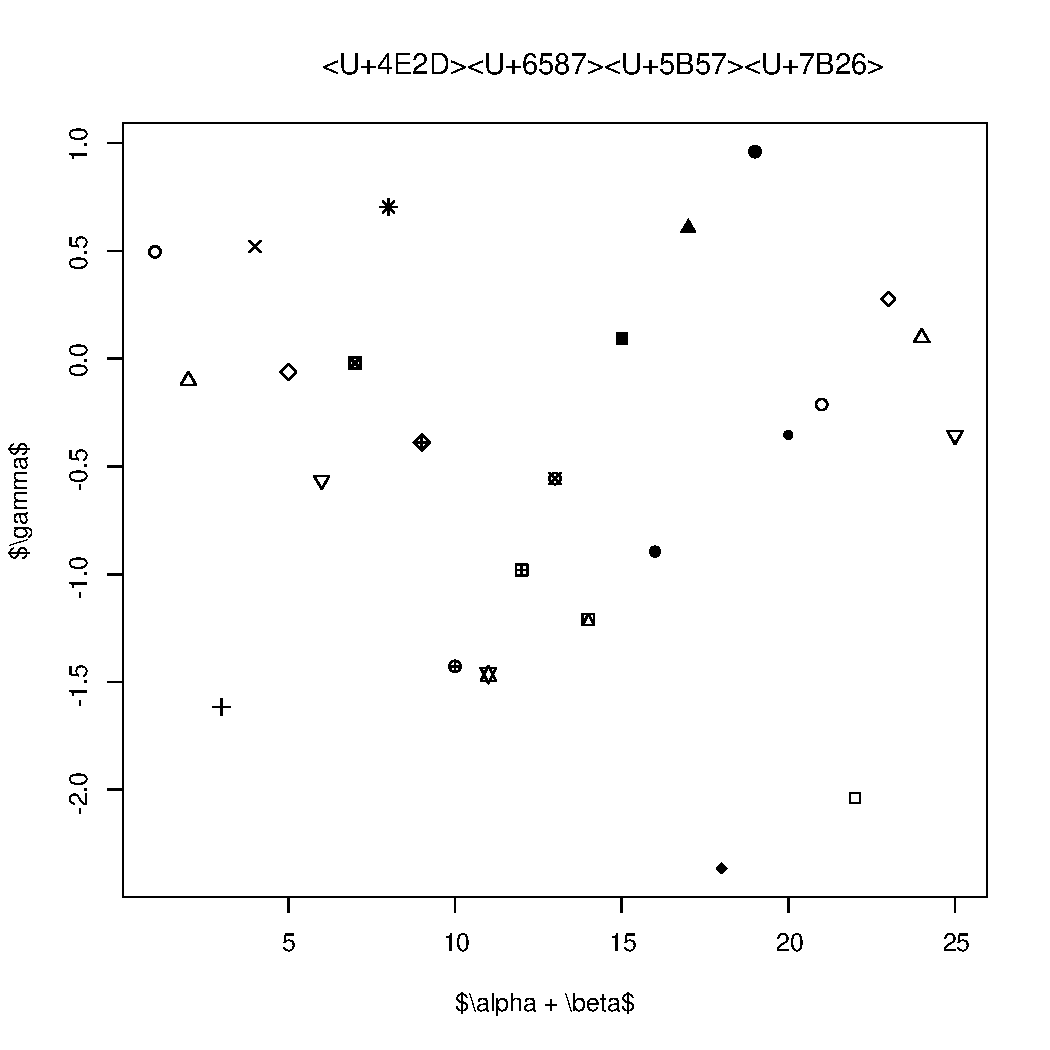
\includegraphics[width=\maxwidth]{figure/rnorm-1} 

\end{knitrout}
\end{center}
\caption{一幅pgfSweave图}
\end{figure}
\end{CJK}
\end{document}
